\section{Cleaning Techniques}
\noindent The images obtained from the two different datasets had different specifications. While the FFHQ \cite{FFHQ} dataset images were coloured and of size 128*128, the IMDB-WIKI \cite{IMDBWiki} were of varied size and resolution. Thus, all the images had to go through data augmentation. These included,
\begin{itemize}
    \item  Resizing all the images to the same width and height (150 * 150)
    \item Converting all the images to greyscale
    \item Normalizing the brightness of all images to be in the range of 0.5 - 1.5 
    \item Applying a small crop factor to isolate the subject from the background
\end{itemize}

\lstset{
  language=Python,
  basicstyle=\ttfamily,
  numbers=left,
  frame=single,
  captionpos=b,
}

\begin{lstlisting}[caption={Augmenting the dataset using Keras \cite{Keras}}]
train_datagen = ImageDataGenerator(
    width_shift_range=0.2,
    height_shift_range=0.2,
    zoom_range=0.2,        
    fill_mode='nearest',
    featurewise_center=True,
    featurewise_std_normalization=True,
    brightness_range=[0.5, 1.5] 
)
\end{lstlisting}

\hspace*{1em}
\section{Challenges}
\noindent Some of the augmentation techniques could impact a small subset of images which are already well-defined. For example - cropping a well-defined image may lead to losing some information on the subject.\\

\pagebreak
\section{Examples}
\noindent The image below has better isolation from the background post data augmenting. It also helps in bringing out the emotion on display.
\begin{figure}[h!]
    \centering
  
    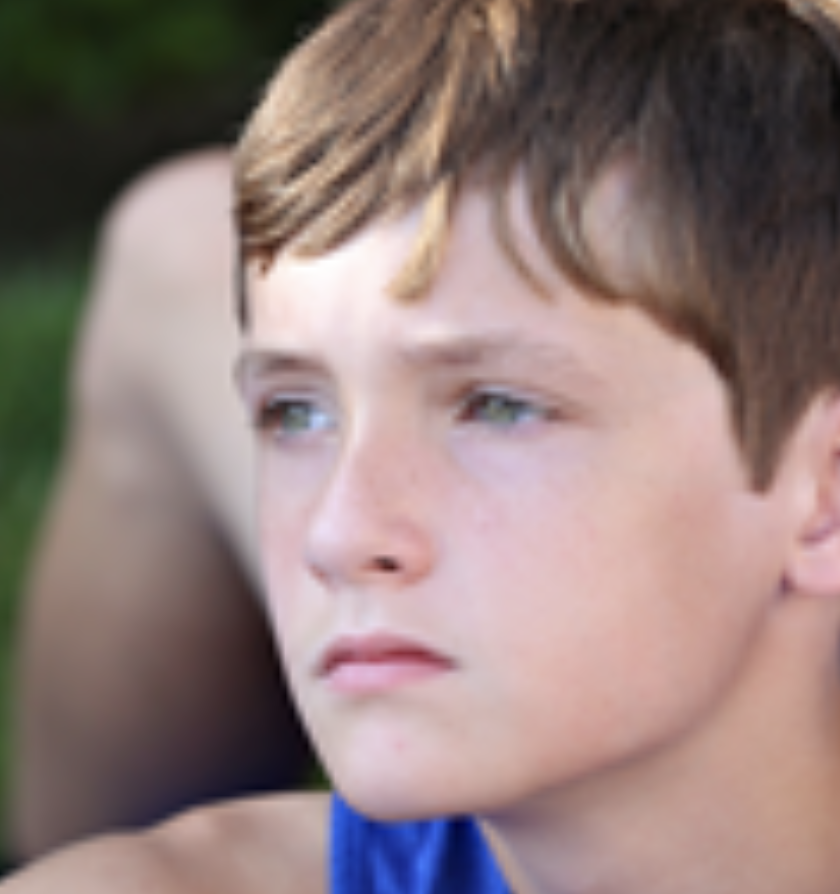
\includegraphics[width=0.3\textwidth, height=5cm]{resources/focus_colour.png} \hspace{3em}
    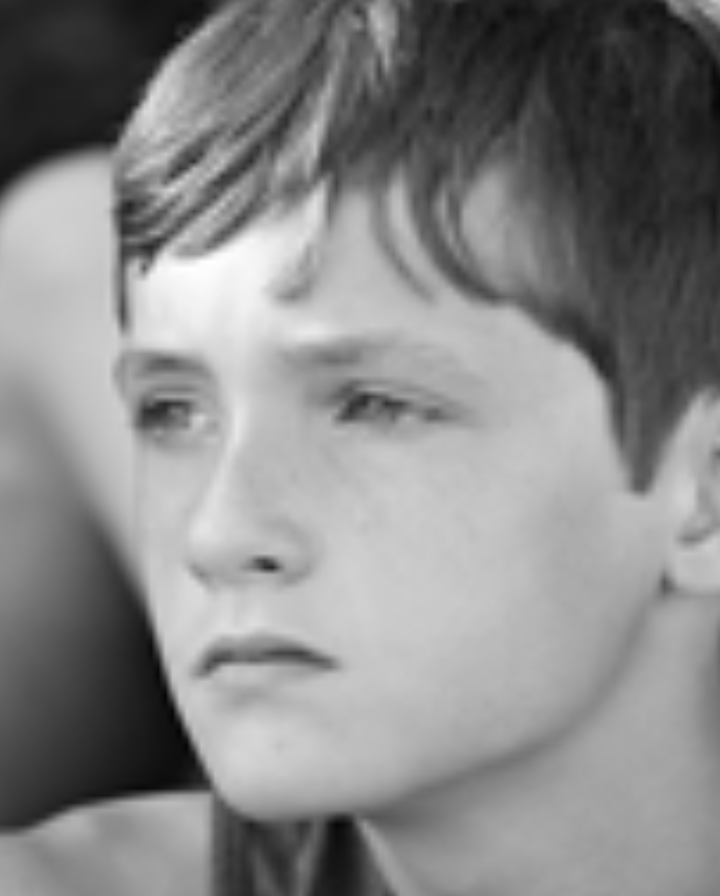
\includegraphics[width=0.3\textwidth, height=5cm]{resources/focus_bw.png}
  
    \caption{Before and after data augmentation}
  \end{figure}